\chapter{Theoretische Grundlagen}
\label{chap:theoretischegrundlagen}

\section{Model Predictive Control}
\label{chap:mpc}


\acrlong{mpc} an sich ist eine Methodik zur Steuerung von Systemen. Diese versucht zunächst, zu sich periodisch wiederholenden, diskreten Zeitpunkten das Verhalten eines Systems in der Zukunft -- also einer immer gleich weit in die Zukunft hineinreichenden Periode -- zu beschreiben. Hierzu bedient \acrlong{mpc} sich der Kenntnis des aktuellen Zustandes und eines physikalischen-mathematischen Modells des Systems, um dessen zukünftiges Verhalten \Gun vorherzusagen \Gob bzw. abzubilden. Des Weiteren wird versucht das Verhalten des Systems mit minimalem Aufwand zu beeinflussen, um einem eigens- oder vordefinierten Zielkriterium zu folgen \acrlong{bzw} diesem zu entsprechen.




\section{Technische Grundlagen zur Kommunikation mit Bussystemen}
\label{sec:grundlagenbus}
In diesem Kapitel werden die Grundlagen von Hard- und Software beleuchtet die für die Kommunikation der Steuerung mit den einzelnen Anlagenteilen benötigt werden.
Diese umfassen zunächst Bussysteme im Allgemeinen und werden anhand des spezifischen/konkreten Anwendungsfalls Modbus erläutert.
Die Einführung wird sich an die Strukutr nach \cite{schn06} anlehnen.

\subsection{OSI-Kommunikationsmodell}
Hier wird das OSI mit Schichten--> Referenzieren von Schichten in den Folgenden.

\subsection{Modbus}
Hier wird das Modbusprotokoll nach \cite{mod12} und \cite{mod06ser} und \cite{mod06tcp}  
Und nach hier wird das Modbusprotokoll nach \cite[S.5]{mod12} und \cite[S.5]{mod06ser} und \cite[S.5]{mod06tcp}

\subsection{Bussysteme} 
Um ganz allgemein Prozesse überwachen und steuern zu können müssen unter den einzelnen Einheiten innerhalb eines Systems Informationen ausgetauscht werden. Dazu werden Kommunikationssysteme benötigt mit Hilfe derer Kommunikation erfolgen kann. Diesem Zweck dienen Bussysteme
Info/Quelle 
%%W. Kriesel, T. Heimbold, D. Telschow: Bustechnologien für die Automation, Hüthig GmbH, Heidelberg 1998
Bussysteme lassen sich anhand verschiedener Kriterien einteilen bzw klassifizieren. Im Rahmen dieser Arbeit wird der Modbus eingesetzt weshalb im Folgenden die Kriterien zunächst sehr allgemein zum Verständnis des Krieteriums beschrieben werden. Die verschiedenen Ausprägungen der einzelnen Kriterien werden lediglich die für Modbus relevanten detailliert beschrieben.

\subsection{Netzwerk und Topologie}
Verknüpft man einzelne Prozesseinheiten -- im folgenden Teilnehmer des Netzwerks -- miteinander über Verbindungsleitungen, über die Informationen übertragen werden können, entstehen dabei Netzwerke. Diese Netzwerke können unterschiedlich ausgeprägt sein und werden anhand ihrer geometrischen Anordnung, der Netzwerktopologie, unterschieden.
--> Teilnehmer im Netzwerk definieren

Die einfachste Art zwei Teilnehmer miteinander zu verbinden ist eine direkte Zweipunktverbindung mit einer Leitung. Jedoch würde mit jeder steigenden Zahl von Teinehmern auch überproportional mehr Verbindungsleitungen benötigt um alle Teilnehmer miteinander zu verbinden. Dies hätte für große Zweipunbktverbindungsnetzwerke. die auch als vermaschtes Netz bezeichnet werden, eine unübersichtliche große Anzahl von Schnittstellen, einen extrem hohen Verkabelungsaufwand und damit verbundene hohe Kosten zur Folge. Um dies zu vermeiden ergeben sich noch verschiedene andere Möglichkeiten zur Anordnung von Teilnehmern in Netzwerken \cite[S.~1f.]{schn06}.

Die Zweipunktverbindungen sind wie oben beschrieben mit einem hohen Verkabelungsaufwand verbunden, weshalb bei großen Netzwerken oftmals zu einer Linienstruktur übergegangen wird. Diese wird auch Linienstruktur genannt und wird auch von der Modbus-Technologie empfohlen/vorgeschrieben. Charakteristisch dafür ist, dass alle Teilnehmer eine gemeinsame Verbindungsleitung zur Kommunikation nutzen. Dazu gibt es ein sogenanntes, langes Buskabel entlang dessen die einzelnen Teilnehmer mit Hilfe von kurzen Stichleitungen angebunden sind, wie auf Abbildung \ref{fig:bus_struktur} zu sehen ist.

\begin{figure}
\centering
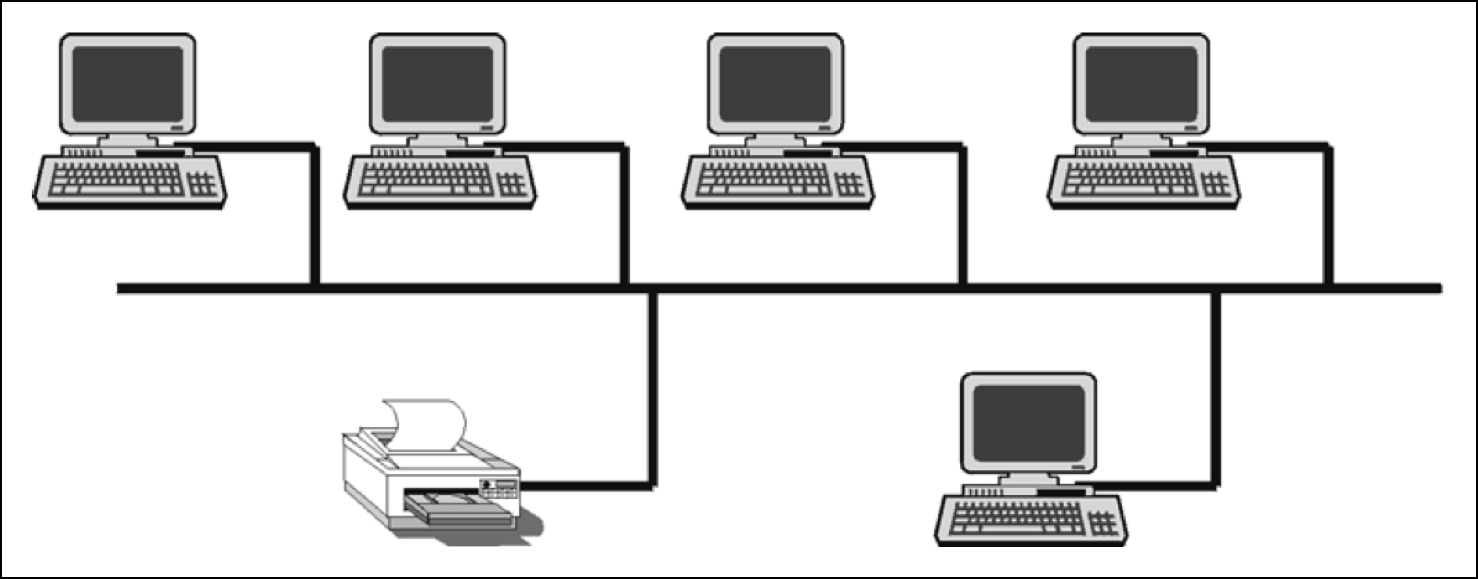
\includegraphics[width=\textwidth]{abbildungen/20160109_busstruktur}
\caption[Linienstruktur]{Linienstruktur aus \cite[S.~3]{schn06}}
\label{fig:bus_struktur}
\end{figure}

Dadurch wird der Verkabelungsaufwand auch für sehr große Netzwerke stark reduziert und auch die Anzahl an Schnittstellen der Teilnehmer auf eine einzige reduziert. Jedoch wird dadurch das gleichzeitige Senden von Teilnehmern erschwert und es müssen sogenannte Buszugriffsverfahren definiert werden, die nichts weiter als Regeln sind die den Zugriff auf den Bus festlegen. Da die Kommunikation auf einer einzigen Leitung stattfindet und ständig alle Teilnehmer alle Sendungen verfolgen wird der Sender durch diese Parallelschaltung der Empfänger stark belastet. Da die Bus-Längen meist sehr lang sind ( hunderte Meter) ist die Leitungslänge im Bezug auf die zu übertragende Wellenlänge nicht mehr vernachlässigbar. Deshalb müssen beide Enden der Busleitung mit Leitungsabschlusswiderständen versehen werden sowie die Leitungslänge und die Teilnehmer je Netzwerk begrenzt werden. Der Leistungs- und Kapazitätswiderstand einer Leitung sind von der Länge der Leitung abhängig und werden durch das Ersatzschaltbild eines RC-Gliedes repräsentiert, wie in Abbildung \ref{fig:bus_impuls}a zu sehen ist. Durch diese Widerstände wird eine Impulsverzerrung $\delta t$ auf der Leitung ausgelöst, die somit mittelbar auch von der Leitungslänge abhängt. Je länger die Leitung desto größer die beiden Widerstande und desto größer ist die Impulsverzerrung $\delta t$, da der Kondensator C\_{Leitung} mehr Zeit zum Aufladen benötigt und die Lastspannung sinkt, wie in Abbildung \ref{fig:bus_impuls}b und \ref{fig:bus_impuls}c dargestellt. Dadurch wird die maximale Frequenz der Datenübertragung beschränkt (auf den Kehrwert der Impulsverzerrung f=1/t). Dies bedeutet das die Frequenz der Datenübertragung entlang der Leitung von ihrer Länge mittelbar abhängig ist, da ansonsten der Empfänger den Wechsel des logischen Zustand nicht mehr registrieren kann \cite[S.~3ff.]{schn06}.

\begin{figure}
\centering
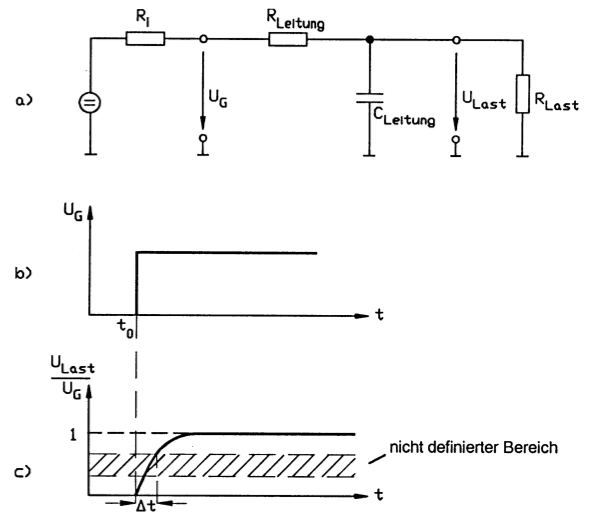
\includegraphics[width=0.6\textwidth]{abbildungen/20160110_impulsbus}
\caption[Impulsverzerrung auf einer Leitung]{Impulsverzerrung auf einer Leitung: a) Ersatzschaltbild der Anordnung b) Ausgangsspannung des Generators c) Empfängerspannung aus \cite[S.~4]{schn06}}
\label{fig:bus_impuls}
\end{figure}

Weitere Bus-Strukturen sind die Baumstruktur, die eine Weiterentwicklung der Linienstruktur ist und auf Abbildung \ref{fig:baum_struktur}. Dabei werden einzelne Linienstrukturen durch Verstärkerelemente, sogenannte  Repeater, miteinander verbunden und es können dadurch größere Flächen als mit der Linienstruktur vernetzt werden. \cite[S.5~f.]{schn06}.
--> Galvanische Trennung und Abschirmung 
Diese Struktur ist insofern interessant, da es also im Rahmen dieser Arbeit Anlage noch eine nachträgliche Erweiterung/Vergrößerung der geplanten Anlage ermöglicht.

Modbus was da oben steht, Teilnehmer kabellängen etc.

\begin{figure}
\centering
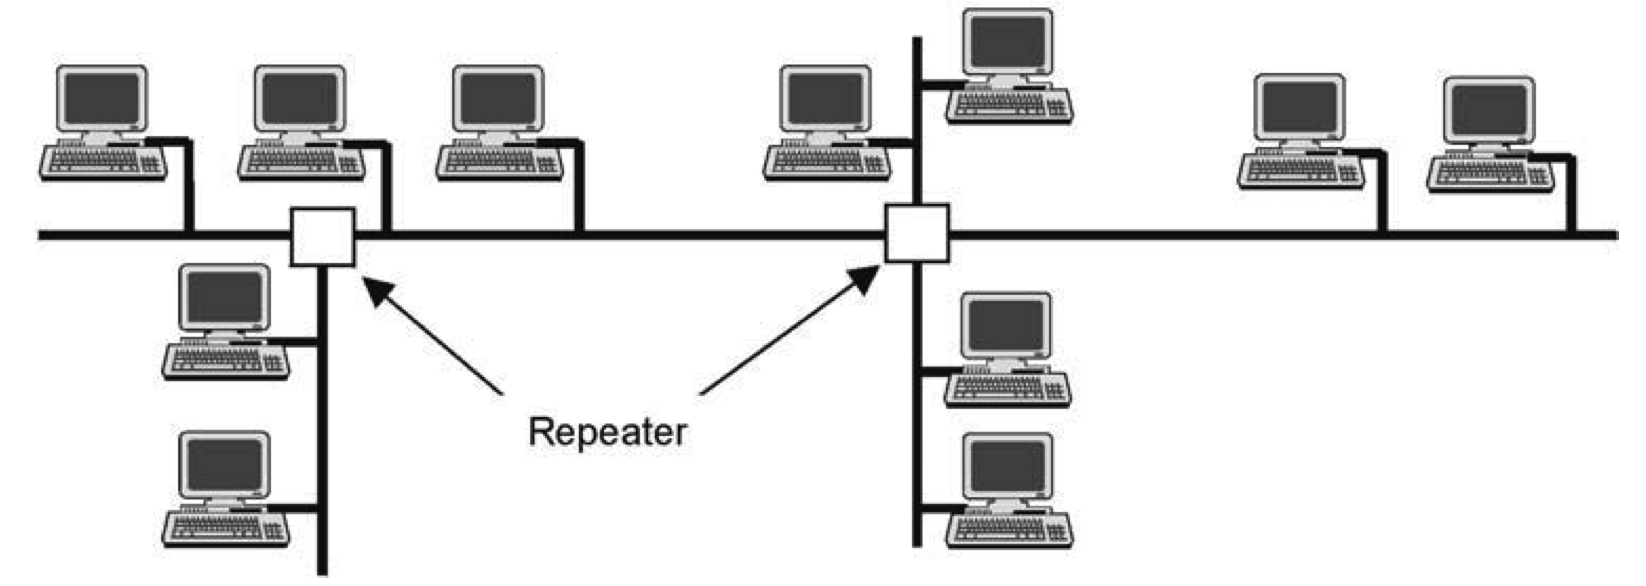
\includegraphics[width=\textwidth]{abbildungen/20160110_baumstruktur}
\caption[Baumstruktur]{Baumstruktur aus \cite[S.~5]{schn06}}
\label{fig:baum_struktur}
\end{figure}

Weitere wichtige Netzwerk Topologien, die für das Verständnis dieser Arbeit keine weitere Relevanz haben, jedoch genannt werden sollten sind die Ring- und die Stern-Struktur. Die Ring-Struktur ist dadurch gekennzeichnet, ein physikalischer Ring mit Zweipunktverbindungen aufgebaut wird in dem über Teilnehmer hinweg kommuniziert wird. Die Stern-Topologie ist durch eine Zentralstation gekennzeichnet, die mit allen Teilnehmer verbunden ist und über die die gesamte Kommunikation abläuft \cite[S.~6f.]{schn06}.



\subsubsection{Elektrisches EIA-485 Netzwerk/Interface}
Hier wird EIA / RS485 dargestellt und abgegrenzt zu RS 232 und RS 422

\subsubsection{Hardware}
Kabel, Belegung







\section{Technische Grundlagen zur Modellbildung}
\label{sec:grundlagenmodell}
In diesem Kapitel werden die technischen Grundlagen zur Bilanzierung, welche für die Modellbildung benötigt werden, erläutert.

\subsection{Thermodynamische Systeme}
Im Raummodell müssen Energieströme, genauer betrachtet Wärmeströme, untersucht werden. Um diese mit Hilfe von Bilanzierungen zu beschreiben folgt zunächst ein kurze Einführung in die Thermodynamische Systembildung nach \cite[S.~11ff.]{ba12}.


Die thermodynamischen Systeme sind dadurch charakterisiert, dass sie durch den zu untersuchenden Raum abgegrenzt sind. Sie dienen dem Zweck der Bilanzierung von Massen- und Energieströmen. Alles was diesen abgegrenzten Raum an den Systemgrenzen umgibt wird als Umgebung bezeichnet. Die begrenzenden Flächen können gedanklicher, physischer oder beider Natur sein, sie müssen lediglich eindeutig festgelegt sein.
Anhand der Eigenschaften der Systemgrenzen lassen sich die Systeme weiter differenzieren.
Bei Systemen deren Grenzen undurchlässig für Materie sind spricht man von geschlossenen Systemen. Die Grenzen eines solchen Systems sind meistens räumlich fest/definiert, müssen aber nicht gezwungenermaßen räumlich fest/fix sondern könne auch beweglich sein und werden dann durch das Volumen der Stoffmenge festgelegt.
Sind die Grenzen für Materie durchlässig spricht man von offenen Systemen die in der Regel durch räumlich festgelegte räumliche Grenzen begrenzt sind. Dieser wird auch als Kontrollraum zbw. Kontrollvolumen bezeichnet. Diese werden können von Stoffströmen durchflossen werden.
Ein abgeschlossenes System umfasst in der Regel mehrere Systeme \acrlong{bzw} ein System und dessen Umgebung sodass es zwischen dessen Grenzen und der Umgebung des abgeschlossenen Systems keine Wechselwirkungen gibt, dass heißt über dessen Grenzen hinweg fließen keine bzw. keine relevanten, dh kaum messbare, Flüsse von Materie und Energie.


Solche thermodynamischen Systeme werden durch physikalische Größen beschrieben, welche gleichzeitig seine Eigenschaften kennzeichnen. Im Rahmen dieser Arbeit ist es ausreichend die Vorgänge und Effekte auf Makroskopischer Ebene zu betrachten, daher lässt sich ein solches Systems mit wenigen Variablen/Größen beschreiben.
Deshalb wird innerhalb der Grenzen eines thermodynamischen Systems, also auch implizit für das Raummodell(Diese Annahme ist noch zu überprüfen und zu diskutieren), angenommen werden, dass die physikalischen Eigenschaften wie z.B. Temperatur, Druck und die chemische Zusammensetzung homogen ist, also an jeder Stelle die gleiche Ausprägung besitzt \cite[S.15]{ba12} . 
Die Variablen lassen sich in äußere, welche den mechanischen Zustand beschreiben (Koordinaten im Raum, relative Geschw. zum Beobachter), und innere, welche den thermodynamischen Zustand der MAterie innerhalb der Systemgrenzen beschreiben , Größen aufteilen.
Der Zustand eines Systems wird also durch die Variablen die ihn beschreiben charakterisiert/definiert, welshalb die Variablen, wie auch im Folgenden, als Zustandsgrößen bezeichnet werden.
\cite[S.13~f.]{ba12}


Da wir im Rahmen von \acrlong{mpc} Zustände und deren Änderungen untersuchen müssen auch Zustandsänderungen untersucht werden. Zustandsänderungen eines Systems werden durch Änderungen (also Flüsse) von Energie und Materie/Masse über dessen Grenzen hinweg bedingt. Diese finden meist im Austausch der Umgebung statt. Während einer solchen Änderung des Systemzustands wird ein Prozess durchlaufen, der eine zeitliche Abfolge von Ereignissen ist. Eine gleiche Zustandsänderung kann also durch verschiedene Prozesse bewirkt werden. Ein Prozess beschreibt also mehr als die reine Zustandsänderung des Systems sondern viel mehr die Beziehungen zwischen einem System und seiner Umgebung. 
Ein Prozess ist also umfassender als eine Zustandsänderung und diese weist lediglich auf einen ablaufenden Prozess hin.
Ein Prozess kann aber auch innerhalb eines Systems ohne äußere Einwirkungen stattfinden, z.B. durch Aufheben innnerer Hemmungen oder Zwängen von Außen. Dies sind meist von selbst statfindende Prozesse in abgeschlossenen Systemen, wie auch relevant für die Modellbildung in Kapitel \ref{chap:modellbildung}. Diese Prozesse werden Ausgleichsprozesse genannt, die danach streben einen Gleichgewichtszustand als Endzustand einzunehmen(\Gun Erfahrungsatz\Gob dass ein sich selbst überlassenes abgeschl. System einem GG-Zustand zustrebt). Solche Ausgleichprozesse repräsentieren Wechselwirkungen zwischen verschiedenen Teilen des abgeschlossenen Systems, die dabei versuchen die Zustandsgrößen auszugleichen und in den GG-Zustand zu kommen, in dem das System vsich von sich aus nicht ändert sondern nur durch äußere Eingriffe, da das System den GG nie von selbst verlässt. Ein abgeschlossenes System strebt also imme einem GG-Zustand hinterher, der durch die Zustände in den einzelnen Teilen(Subsystemen) bestimmt wird. 
\cite[S.21~f.]{ba12}

Reversible Prozesse, da angenommen dass Umgebung groß genug damit die \Gun kleinen\Gob Energieströme vernachlässigt werden können. -notwendig?!


\subsection{Erster Hauptsatz der Thermodynamik}

\cite[S.~43ff.]{ba12}
Der erste Hauptsatz der Thermodynamik erweitert den mechanischen Ernergieerhaltungssatz um die Energieformen Wärme und Energie und handelt ganz allgemein vom Prinzip der Energieerhaltung und dient der Bilanzierung von Systemen und wird später bei der Modellbildung des Raumes Anwendung finden. 
Die Energie eines Systems $E$ besteht aus potenzieller $E_{pot}$ und kinetischer Energie $E_{kin}$ wie in der Mechanik und wird durch die Innere Energie $U$ ergänzt wie in nachstehender Gleichung beschrieben \cite[S.~49]{ba12}

\begin{equation}
\label{eq:energie}
E := E_{pot} + E_{kin} + U
\end{equation}
 
Die mechanischen Energie kann bei den nachfogenden Betrachtungen vernachlässigt werden, da es sich um ein ortsfestes System handelt, das heißt die potentielle Energie ist konstant, in das und aus dem heraus keine Ströme fließen und es sich eslbts nicht bewegt, das heißt die kinetsiche Energie bleobt evenfalls kosntant und können somit beide vernachlässigt werden und die Energie des Systems wird verinfacht nur durch durch die innere Energie angenommen.



Die innere Energie ist abhängig von der spezifischen Wärmekapazität und der Masse innerhalb eines Systems und berechnet sich nach der veränderten Gleichung aus \cite[S.~54]{ba12} und entspricht der Energie der Masse eines Systems:

\begin{equation}
\label{eq:innereenergie}
U := m*c_p*T bzw. m*c_p*(t-T_0)+u_0
\end{equation}

Erst qualitativ, dann quantitaiv
Der 1. Hauptsatz besagt, dass jedes System eine Energie als Zustandsgröße besitzt die sich aus den folgenden zusammensetzt:
mechanisch
wärme
innere Energie

\cite[S.~48]{ba12}
Außerdem kann sich energie nur durch transport über die grenzen hinweg ändern und es gilt das prinzip der nergieerhaltung. Möglich trabsportformen, Verricgten von arbeit --> wie mechanik, d.h. umewandlung von enegrie
Übergang von wärme, das heiosst qärmetrabsprot, und Transport von Materie, da Mateire gleiche energie, also auch durch Stoffstransport.
Daraus kfolgt die Energiebilanzgleichung um den effekt quanititiv zu bescheibeen
Energie System Gesamt E= Ekin+Epot+U --Y Auch System in Ruhe, d.h. ekin=epot=0 hat Energie
U ist innere Energie und ebschreibt die Energie die innerhalb eines Systems, durch bestandteile und ist abhönigg von der der masse, da Masse=energie
Energie eines systems ist konstant und berechnet sich nach folgender Gleichung \cite[S.~54]{ba12}

\begin{equation}
\label{eq:hauptsatz}
Q_{12} + W_{12} = E_2 - E_1
\end{equation}


\subsection{Wärmeübertragung}
Da zur Betsimmung und Steuerung einer Raumheizungsnalage die Betrachtung von Wärmeströmen unumgänglich ist werden die Grundlagen dazu im Folgenden erläutert.
Die Wärmeübertragung kann grundsätzlich nur durch zwei Arten stattfinden, durch Strahlung, die ohne stofflichen Träger durch elektromagnetische Wellen erfolgt, welche keine weitere Relevanz für weitere Betrachtungen hat und deshalb hier nicht erläutert wird, und durch die Wärmeleitung, die sich wiederum in die Leitung und die Konvektion aufteilt. \cite[S.~3f.]{bo14}

Die Wärmeübertragung wird druch den Wärmestrom $\dot{Q}$ beschrieben, der quantifiziert wieviel Wärme pro Zeiteinheit $[W]$ übertragen wird \cite[S.~5]{bo14}.
Für die weitere Betrachtung im Rahmen dieser Arbeit ist lediglich die Wärmeleitung ohne KOnvektion von Relevanz, weshalb diese nun näher erläutert wird.
Kinetische Kopplungsgleichung\cite[S.~7]{bo14}
Gleichung Qdot =k*A*deltaT
Geben Wärmestrom als Funktion an von verschiedenen Paramatern, hier Fläche an der Austausch stattfindet, Temperaturdifferenz und Wärmedurchgangszahl bzw Wärmeübergangszahl an.
Wärmedurchgangskoeefizient oder auch U Wert
Übertsragung folgt ab Seite 17 Wärmebuch
